\documentclass[11pt]{article}
\usepackage[margin=2.5cm]{geometry}
\usepackage{amsmath, amssymb}
\usepackage{booktabs}
\usepackage{xcolor}
\usepackage{listings}
\usepackage{graphicx}
\usepackage{hyperref}

\lstset{
  language=Python,
  basicstyle=\ttfamily\small,
  keywordstyle=\color{blue!70!black}\bfseries,
  commentstyle=\color{green!45!black},
  stringstyle=\color{red!60!black},
  frame=single,
  breaklines=true,
  columns=fullflexible,
  showstringspaces=false
}

\title{Quantile Regression with a Neural Network in PyTorch}
\author{}
\date{}

\begin{document}
\maketitle

\section{What Is a Quantile?}

Let $Y$ be a random variable with cumulative distribution function
$F_Y(y) = P(Y \le y)$. For a level $q \in (0,1)$, the \emph{$q$-th quantile}
of $Y$ is the value below which a fraction $q$ of the probability mass lies:
\[
  Q_Y(q) = \inf\{\, y : F_Y(y) \ge q \,\}.
\]
Intuitively, $Q_Y(q)$ answers the question: \emph{``what value is $Y$ below
  $100q\%$ of the time?''}

\begin{itemize}
  \item $q = 0.5$ gives the \textbf{median}: half the outcomes are below it, half above.
  \item $q = 0.1$ gives the 10th percentile: only 10\% of outcomes fall below it.
  \item $q = 0.9$ gives the 90th percentile: 90\% of outcomes fall below it.
\end{itemize}

For example, if $Y \sim \mathcal{N}(\mu, \sigma^2)$, then
$Q_Y(q) = \mu + z_q\,\sigma$, where $z_q$ is the standard normal quantile
($z_{0.1} \approx -1.28$, $z_{0.5} = 0$, $z_{0.9} \approx 1.28$).

In regression we care about the \emph{conditional} quantile
$Q_{Y \mid X}(q \mid x)$: the $q$-th quantile of $Y$ given that the input is $x$.
The pair $\big(Q_{Y\mid X}(0.1\mid x),\; Q_{Y\mid X}(0.9\mid x)\big)$ forms an
80\% prediction interval for $Y$ at input $x$.

\section{Linear Regression vs.\ Quantile Regression}

\subsection{Linear (least-squares) regression}

Ordinary least-squares regression fits a model $\hat y = f(x)$ by minimizing
the mean squared error:
\[
  \min_f \; \frac{1}{N}\sum_{i=1}^{N} \big(y_i - f(x_i)\big)^2 .
\]
The minimizer of the squared error is the \textbf{conditional mean}
$\mathbb{E}[Y \mid X = x]$. Hence least-squares regression produces a
\emph{single number} per input: the average outcome. It says nothing about how
spread out the outcomes are around that average.

\subsection{Quantile regression}

Quantile regression replaces the squared error with the \emph{pinball loss}
(Section~\ref{sec:pinball}). Its minimizer is the \textbf{conditional quantile}
$Q_{Y\mid X}(q \mid x)$. By fitting several quantiles at once we obtain a
picture of the whole conditional distribution, not just its centre.

\subsection{Key differences}

\begin{center}
  \begin{tabular}{@{}lll@{}}
    \toprule
                      & \textbf{Least-squares regression} & \textbf{Quantile regression}  \\
    \midrule
    Loss              & Squared error $(y-\hat y)^2$      & Pinball loss $L_q(y,\hat y)$  \\
    Estimates         & Conditional mean                  & Conditional $q$-quantile      \\
    Outputs per input & One value                         & One value per quantile level  \\
    Uncertainty       & Not captured                      & Prediction intervals          \\
    Outliers          & Sensitive (errors squared)        & Robust (errors linear)        \\
    Noise assumption  & Usually constant variance         & None; handles changing spread \\
    \bottomrule
  \end{tabular}
\end{center}

\paragraph{A note on ``linear''.}
``Linear'' refers to the form of the model, $f(x) = w^\top x + b$, while
``least squares'' and ``quantile'' refer to the loss. Linear quantile
regression also exists (a linear model trained with pinball loss). In this
project the model is a \emph{neural network}, so it can learn non-linear
quantile curves such as $3\sin(x)$.

\section{The Pinball Loss}
\label{sec:pinball}

\subsection{Definition}

Define the residual (error)
\[
  e = y - \hat y,
\]
where $y$ is the true label and $\hat y$ the prediction. A positive $e$ means
the model \emph{under-predicted}; a negative $e$ means it
\emph{over-predicted}. The pinball loss for quantile level $q$ is
\[
  L_q(y, \hat y) =
  \begin{cases}
    q\,(y - \hat y)     & \text{if } y \ge \hat y, \\
    (1-q)\,(\hat y - y) & \text{if } y < \hat y.
  \end{cases}
\]

\subsection{From the formula to a single expression}

Substituting $e = y - \hat y$, the second case becomes
$(1-q)(-e) = (q-1)\,e$, so
\[
  L_q =
  \begin{cases}
    q\,e     & e \ge 0, \\
    (q-1)\,e & e < 0.
  \end{cases}
\]
Because $0 < q < 1$, the factor $q$ is positive and $q-1$ is negative.
Therefore $q\,e$ and $(q-1)\,e$ always have opposite signs, and the correct
branch is always the non-negative one:

\begin{center}
  \begin{tabular}{@{}lccc@{}}
    \toprule
    Case                         & $q\,e$  & $(q-1)\,e$ & Maximum    \\
    \midrule
    $e \ge 0$ (under-prediction) & $\ge 0$ & $\le 0$    & $q\,e$     \\
    $e < 0$ (over-prediction)    & $< 0$   & $> 0$      & $(q-1)\,e$ \\
    \bottomrule
  \end{tabular}
\end{center}

This gives the branch-free form used in code:
\[
  \boxed{\,L_q(y,\hat y) = \max\big(q\,e,\; (q-1)\,e\big)\,}
\]

\subsection{Why it produces quantiles}

For $q = 0.9$, under-predicting costs $0.9\,|e|$ while over-predicting costs
only $0.1\,|e|$. The model is pushed upward until only about 10\% of targets
lie above its prediction, which is exactly the 90th percentile. For $q = 0.5$
both sides cost the same, the loss equals $\tfrac12|e|$, and the minimizer is
the median.

\subsection{Gradient}

With respect to the prediction,
\[
  \frac{\partial L_q}{\partial \hat y} =
  \begin{cases}
    -q    & e > 0, \\
    1 - q & e < 0.
  \end{cases}
\]
The loss is not differentiable at $e = 0$; PyTorch's \texttt{torch.max} simply
picks one branch there, which works fine in practice. Note that the gradient
does not shrink as $e \to 0$ (unlike squared error), which is why pinball loss
tends to need more training epochs.

\section{Implementation, Step by Step}

The notebook is described cell by cell, in execution order.

\subsection{Step 1: Imports}

\begin{lstlisting}
import torch
import torch.nn as nn
import torch.optim as optim
from torch.utils.data import TensorDataset, DataLoader
import matplotlib.pyplot as plt
\end{lstlisting}

\begin{itemize}
  \item \texttt{torch}: tensors and automatic differentiation.
  \item \texttt{torch.nn}: neural-network layers.
  \item \texttt{torch.optim}: optimizers such as Adam.
  \item \texttt{TensorDataset}, \texttt{DataLoader}: wrap tensors and serve them in shuffled mini-batches.
  \item \texttt{matplotlib.pyplot}: plotting.
\end{itemize}

\subsection{Step 2: Choosing the device}

\begin{lstlisting}
device = "cuda" if torch.cuda.is_available() else "cpu"
print(device)
\end{lstlisting}

Use the GPU if one is available, otherwise the CPU. All model parameters and
every tensor fed to the model must live on the same device.

\subsection{Step 3: Generating synthetic data}

\begin{lstlisting}
n = 10000
x = torch.rand(n, 1) * 10
noise = torch.randn(n, 1) * (0.1 + 0.3 * x)
y = (torch.sin(x) * 3 + noise).squeeze(1)
loader = DataLoader(TensorDataset(x, y), batch_size=128, shuffle=True)
\end{lstlisting}

The data are generated from
\[
  y = 3\sin(x) + \varepsilon, \qquad
  \varepsilon \sim \mathcal{N}\!\big(0,\; (0.1 + 0.3x)^2\big), \qquad
  x \sim \mathcal{U}(0, 10).
\]

\begin{itemize}
  \item \texttt{x} has shape $(n, 1)$: $n$ samples, one feature each.
  \item The noise standard deviation grows with $x$ (\emph{heteroscedastic}
        noise). This is where quantile regression shines: least squares would
        return only the curve $3\sin(x)$, while the quantile bands widen as
        $x$ grows.
  \item \texttt{.squeeze(1)} removes the size-1 column, so \texttt{y} has shape $(n,)$.
  \item Because the generating process is known, so are the true quantiles:
        $Q(q \mid x) = 3\sin(x) + z_q\,(0.1 + 0.3x)$. The trained model can be
        checked against them.
  \item The \texttt{DataLoader} shuffles the data each epoch and yields
        batches of 128 samples.
\end{itemize}

\subsection{Step 4: The neural network}

\begin{lstlisting}
class NeuralNetwork(nn.Module):
    def __init__(self, in_dim, hid_dim, out_dim):
        super().__init__()
        self.forward_pass = nn.Sequential(
            nn.Linear(in_dim, hid_dim),
            nn.ReLU(),
            nn.Linear(hid_dim, hid_dim),
            nn.ReLU(),
            nn.Linear(hid_dim, out_dim),
        )

    def forward(self, x):
        return self.forward_pass(x)
\end{lstlisting}

\begin{itemize}
  \item \texttt{super().\_\_init\_\_()} initializes the parent
        \texttt{nn.Module}, which is what lets PyTorch track the layers'
        parameters. It takes no arguments: \texttt{super()} already binds
        \texttt{self}.
  \item The network is a multilayer perceptron: two hidden layers of width
        \texttt{hid\_dim} with ReLU activations, mapping
        $\mathbb{R}^{\text{in\_dim}} \to \mathbb{R}^{\text{out\_dim}}$.
  \item \texttt{out\_dim} equals the number of quantiles. Each output neuron
        predicts one quantile, so a single network learns all of them at once
        and they share the hidden features.
\end{itemize}

\subsection{Step 5: The pinball loss}

\begin{lstlisting}
def pinball_loss(prediction, label, quantiles):
    error = label.view(-1, 1) - prediction
    return torch.max(quantiles * error, (quantiles - 1) * error).mean()
\end{lstlisting}

This is the boxed formula from Section~\ref{sec:pinball}, applied to a whole
batch at once. The shapes are:

\begin{itemize}
  \item \texttt{label}: $(N,)$, the true values $y$.
  \item \texttt{prediction}: $(N, Q)$, the predictions $\hat y$ for $Q$ quantiles.
  \item \texttt{quantiles}: $(Q,)$, the levels $q_1,\dots,q_Q$.
\end{itemize}

\paragraph{Reshaping with \texttt{view}.}
\texttt{view} reshapes a tensor without copying its data. In
\texttt{view(-1, 1)}, the \texttt{1} requests exactly one column and the
\texttt{-1} tells PyTorch to infer the number of rows from the total size.
The label therefore becomes a column of shape $(N, 1)$.

\paragraph{Broadcasting.}
Subtracting $(N, Q)$ from $(N, 1)$ stretches the single column across all
$Q$ columns:
\[
  \texttt{error}_{ij} = y_i - \hat y_{ij},
\]
so every sample's label is compared against each of its $Q$ quantile
predictions. Similarly, \texttt{quantiles} of shape $(Q,)$ is broadcast across
rows, so column $j$ is weighted by its own $q_j$. Without the \texttt{view},
an $(N,)$ label would be aligned with the last dimension $Q$, which is wrong.

\paragraph{Reduction.}
\texttt{.mean()} with no arguments averages over all $N \times Q$ entries and
returns a 0-dimensional (scalar) tensor:
\[
  \mathcal{L} = \frac{1}{NQ}\sum_{i=1}^{N}\sum_{j=1}^{Q}
  \max\big(q_j\, e_{ij},\; (q_j - 1)\, e_{ij}\big).
\]
A scalar is what \texttt{loss.backward()} requires. Note that \texttt{.mean()}
returns a scalar even if the shapes are wrong (e.g.\ an $(N,)$ prediction
broadcasts to $(N, N)$), so a shape mistake fails silently rather than with an
error.

\subsection{Step 6: Hyperparameters}

\begin{lstlisting}
quantiles = torch.tensor([0.1, 0.5, 0.9], device=device)
in_dim = 1
hid_dim = 64
out_dim = len(quantiles)
lr = 1e-3
batch_size = 128
epochs = 500
\end{lstlisting}

\begin{itemize}
  \item Quantiles $0.1$, $0.5$, $0.9$: a lower bound, the median, and an upper
        bound, forming an 80\% prediction interval. The tensor is placed on
        \texttt{device} because it is multiplied with GPU tensors in the loss.
  \item \texttt{in\_dim = 1}: one input feature.
  \item \texttt{hid\_dim = 64}: ample capacity for a one-dimensional curve.
  \item \texttt{lr = 1e-3}: the standard Adam learning rate.
  \item \texttt{epochs = 500}: pinball loss converges more slowly than squared
        error because its gradient does not shrink near the optimum.
\end{itemize}

\subsection{Step 7: Training}

\begin{lstlisting}
model = NeuralNetwork(in_dim, hid_dim, out_dim).to(device)
optimizer = optim.Adam(model.parameters(), lr)

for epoch in range(epochs):
    for xb, yb in loader:
        xb, yb = xb.to(device), yb.to(device)
        optimizer.zero_grad()
        loss = pinball_loss(model(xb), yb, quantiles)
        loss.backward()
        optimizer.step()
    if epoch % 50 == 0:
        print(epoch)
\end{lstlisting}

Each iteration over a mini-batch performs:
\begin{enumerate}
  \item \textbf{Move to device}: copy the batch to the GPU.
  \item \textbf{Zero gradients}: PyTorch accumulates gradients by default, so
        the previous step's gradients must be cleared.
  \item \textbf{Forward pass}: compute predictions \texttt{model(xb)} and the
        scalar loss.
  \item \textbf{Backward pass}: \texttt{loss.backward()} uses automatic
        differentiation to compute
        $\partial\mathcal{L}/\partial\theta$ for every parameter $\theta$.
        No hand-written backward pass is needed.
  \item \textbf{Update}: \texttt{optimizer.step()} applies the Adam update to
        the parameters.
\end{enumerate}

\paragraph{Naming pitfall.}
The batch variables are deliberately named \texttt{xb}, \texttt{yb} and not
\texttt{x}, \texttt{y}. Python has no block scope: a \texttt{for} loop assigns
to its variables in the enclosing scope, which in a notebook is the global
scope. Writing \texttt{for x, y in loader} would overwrite the full dataset
with the last mini-batch, which is a GPU tensor.

\subsection{Step 8: Visualizing the result}

\begin{lstlisting}
x, y = loader.dataset.tensors
xs = torch.linspace(0, 10, 200).view(-1, 1)
with torch.no_grad():
    preds = model(xs.to(device)).cpu()

plt.scatter(x, y, s=2, alpha=0.3)
for i, q in enumerate([0.1, 0.5, 0.9]):
    plt.plot(xs, preds[:, i], label=f"q={q}")
plt.legend()
plt.savefig("quantiles.pdf", bbox_inches="tight")
\end{lstlisting}

\begin{itemize}
  \item \texttt{loader.dataset.tensors} recovers the exact (CPU) training data.
  \item \texttt{xs} is a dense grid of 200 points, reshaped to $(200, 1)$ to
        match the model's input shape.
  \item \texttt{torch.no\_grad()} disables gradient tracking, since we are
        only predicting.
  \item \texttt{.cpu()} moves the predictions back to the CPU: matplotlib
        converts tensors to NumPy arrays, which is only possible for CPU
        tensors.
  \item Column $i$ of \texttt{preds} is the curve for quantile $q_i$.
\end{itemize}

\paragraph{What to expect.}
The $q = 0.5$ curve should follow $3\sin(x)$, and the $q = 0.1$ and
$q = 0.9$ curves should form a band that widens as $x$ increases, mirroring the
growing noise. About 10\% of points should lie below the lower curve and about
10\% above the upper one. If two quantile curves cross somewhere, train longer
or sort the outputs per input with \texttt{preds.sort(dim=1).values}.
Figure~\ref{fig:quantiles} shows the result.

\begin{figure}[h]
  \centering
  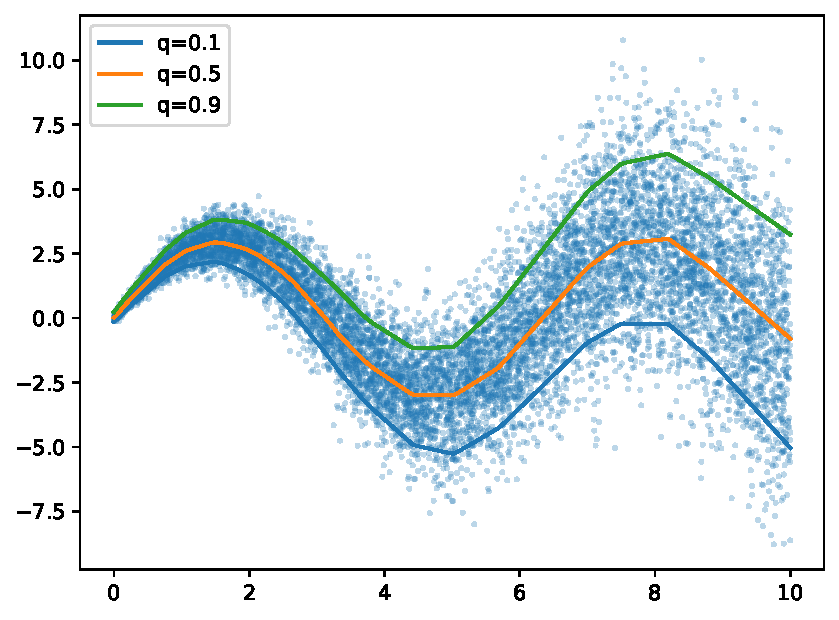
\includegraphics[width=0.8\linewidth]{figures/quantiles.pdf}
  \caption{Training data (blue dots) and the learned conditional quantile
    curves for $q = 0.1$, $0.5$ and $0.9$.}
  \label{fig:quantiles}
\end{figure}

\section{Summary}

\begin{enumerate}
  \item A quantile $Q(q)$ is the value below which a fraction $q$ of outcomes fall.
  \item Least-squares regression estimates the conditional mean; quantile
        regression estimates conditional quantiles and hence the spread of the
        outcomes.
  \item The pinball loss $\max(q\,e, (q-1)\,e)$ penalizes under- and
        over-prediction asymmetrically, and its minimizer is the $q$-quantile.
  \item A single neural network with one output per quantile, trained with
        this loss via autograd and Adam, learns non-linear quantile curves and
        so captures noise whose spread changes with the input.
\end{enumerate}

\end{document}
